%
%  Introduction
%

%-- Chapter Title
\chapter{Introduction}


\begin{quote}

{\em Bayesians are like Vegans, at some point they become impractical.}

\hspace{\stretch{1}} Meetup in the Silicon Valley

\end{quote}


\noindent
 
If a deconfined medium is formed in high-energy heavy-ion collisions, one of its most striking expected characteristics is the suppression of quarkonium states.
This takes place as the force between the constituents of the quarkonium state, a heavy quark and its antiquark, is weakened by the color screening produced by the surrounding light quarks and gluons.
%One of the most triking charateristics associated to quark gluon plasma (QGP) formation  is the suppression of quarkonium states.
%This is thought to be a direct effect of deconfinement, when the force between the constituents of a quarkonium state, a heavy quark and its antiquark, is weakened by the color screening produced by the surrounding light quarks and gluons.
 The suppression is predicted to occur above a critical temperature of the medium, and sequentially, in the
order of the \QQbar binding energy. 
Since the \PgUa is the most tightly bound state among all quarkonia, it is expected to be the one
with the highest dissociation temperature. % in the QGP.
Such a suppression pattern is expected to further depend on complications arising from additional phenomena sometimes referred to as $hot$ and $cold$ nulcear matter effects.This work presented here aims at studying the in detail the bottomonium family of states in ultra-relativistic heavy-ion collisions.   
Given the momentum resolution attained, and the capability of the trigger system,  CMS is unrivaled in the analysis of the upsilon family in the three environemnts studied (pp, pPb and PbPb)



\section{Heavy Ion Physics}

The study of the fundamental theory of the strong interaction --- Quantum Chromodynamics (QCD) ---
in extreme conditions of temperature, density and parton momentum fraction (low-$x$) has
attracted an increasing experimental and theoretical interest during the last 20 years. Indeed,
QCD is not only a quantum field theory with an extremely rich
dynamical content --- such as asymptotic freedom,
infrared slavery, (approximate) chiral symmetry, non-trivial vacuum topology, strong CP violation problem,
U$_A(1)$ axial-vector anomaly, colour superconductivity,
\ldots\ --- but also the only sector of the Standard Model (SM) whose full
{\it collective} behaviour --- phase diagram, phase transitions, thermalisation of fundamental fields ---
is accessible to scrutiny in the laboratory. The study of the many-body dynamics of high-density QCD
covers a vast range of fundamental physics problems (Fig.~\ref{fig:QCD_facets}).

\begin{figure}[htb]
\centering
%\hskip 0.8cm
\includegraphics[width=0.6\textwidth]{introduction/schaefer_qcd_phases}
%\vskip -0.7cm
\caption{Many-body dynamics of QCD in different physics limits.}
%\caption{The multiple facets of QCD.}
\label{fig:QCD_facets}
\end{figure}

\subsection*{Deconfinement and chiral symmetry restoration}

Lattice QCD calculations predict a new form of matter at energy densities
(well) above a critical value ---
$\epsilon_c =(6\pm 2) T_c^4 \approx$ 1 GeV/fm$^3$ (Fig.~\ref{fig:latt_EoS}),
where $T_c\approx$ 150--190 MeV is
the critical temperature --- consisting of an extended volume of deconfined and current-mass quarks
and gluons: the Quark-Gluon Plasma (QGP).


\begin{figure}[htb]
\centering
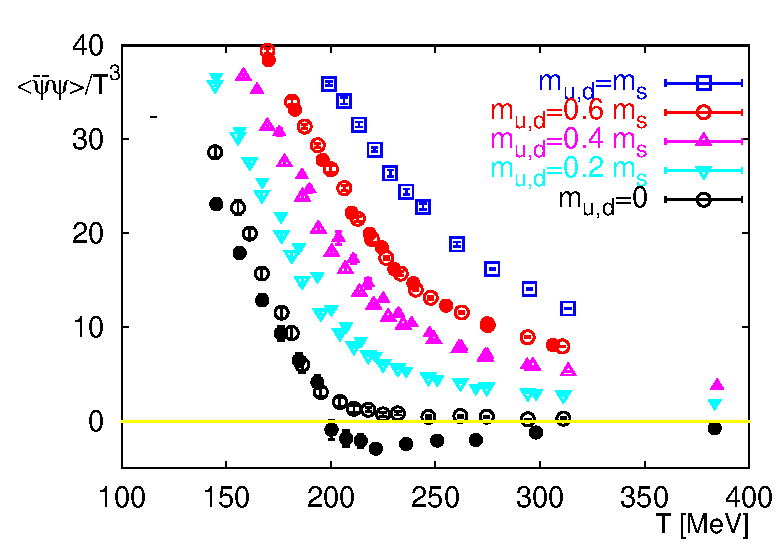
\includegraphics[width=0.48\textwidth]{introduction/latt_qcd_chiral_vs_T}
\includegraphics*[width=0.48\textwidth]{introduction/latt_qcd_EoS}
\caption{Left: The light quark chiral condensate versus the temperature computed in lattice QCD
with various number of flavours and values of the $u,d,s$ quark masses.
Right: The energy density in QCD with 0, 2 and 3 degenerate quark flavours as well as with two light
and one heavier (strange) quarks. %In the case of the SU(3) pure-gauge theory the continuum extrapolated result is shown.
The horizontal arrow shows the value of the Stefan-Boltzmann limit for
an ideal quark-gluon gas}
\label{fig:latt_EoS}
\end{figure}
The vanishing of the chiral condensate at $T_c$ and the sudden liberation of quark and gluon
degrees of freedom are clearly visible in Fig.~\ref{fig:latt_EoS}. The scrutiny of this new state of
matter --- equation-of-state (EoS), order of the phase transition, transport properties, etc. ---
promises to shed light on basic aspects of the strong interaction such as the nature of confinement,
the mechanism of mass generation (chiral symmetry breaking, structure of the QCD vacuum)
and hadronization, which still evade a thorough theoretical description 
due to their highly non-perturbative nature.

In order to calculate physical observables from first principles in QCD it is not enough to
know its Lagrangian. It is also necessary and important to know the true structure of its ground state.
It is just the response of the true QCD vacuum which substantially modifies all the QCD
Green’s functions from their free counterparts.

\subsection*{Parton structure and evolution at small-\texorpdfstring{$x$}{x}}

HERA results indicate that when probed at high energies,
hadrons consist of a very dense system of gluons with small (Bjorken)  momentum
$x=p_{\rm parton}/p_{\rm hadron}$.
At low $x$, the probability to emit an extra gluon is large, proportional to $\alpha_s\ln(1/x)$, and %non-linear
gluon-gluon fusion processes will eventually dominate the parton evolution in the hadronic wavefunctions.
At high virtualities $Q^2$ and moderately low $x$, such evolution %with $Q^2$ (or $\ln(1/x)$)
is described by linear DGLAP or
BFKL equations, suitable for a dilute parton
regime. At $x\lesssim 10^{-2}$, and for $Q$ values below an energy-dependent saturation momentum $Q_s$,
hadrons are however more appropriately
%$Q^2_s \approx\alpha_s\,xG(x,Q^2)/(\pi\,R^2)$, such a configuration
described as dense, saturated parton systems in the context of the ``Colour-Glass Condensate''
(CGC) effective theory with the corresponding non-linear
JIMWLK evolution equations
(Fig.~\ref{fig:CGC_phase_diag}).
%%%Since the growth of the gluon density depends on the transverse size of the hadron,
Low-x gluons in nuclei overlap and, so, saturation effects are expected
to set in earlier for ultrarelativistic heavy nuclei (for which $Q_s^2\propto A^{1/3}$, with $A$
the number of nucleons) than for free nucleons.

\begin{figure}[!Hhtb]
\centering
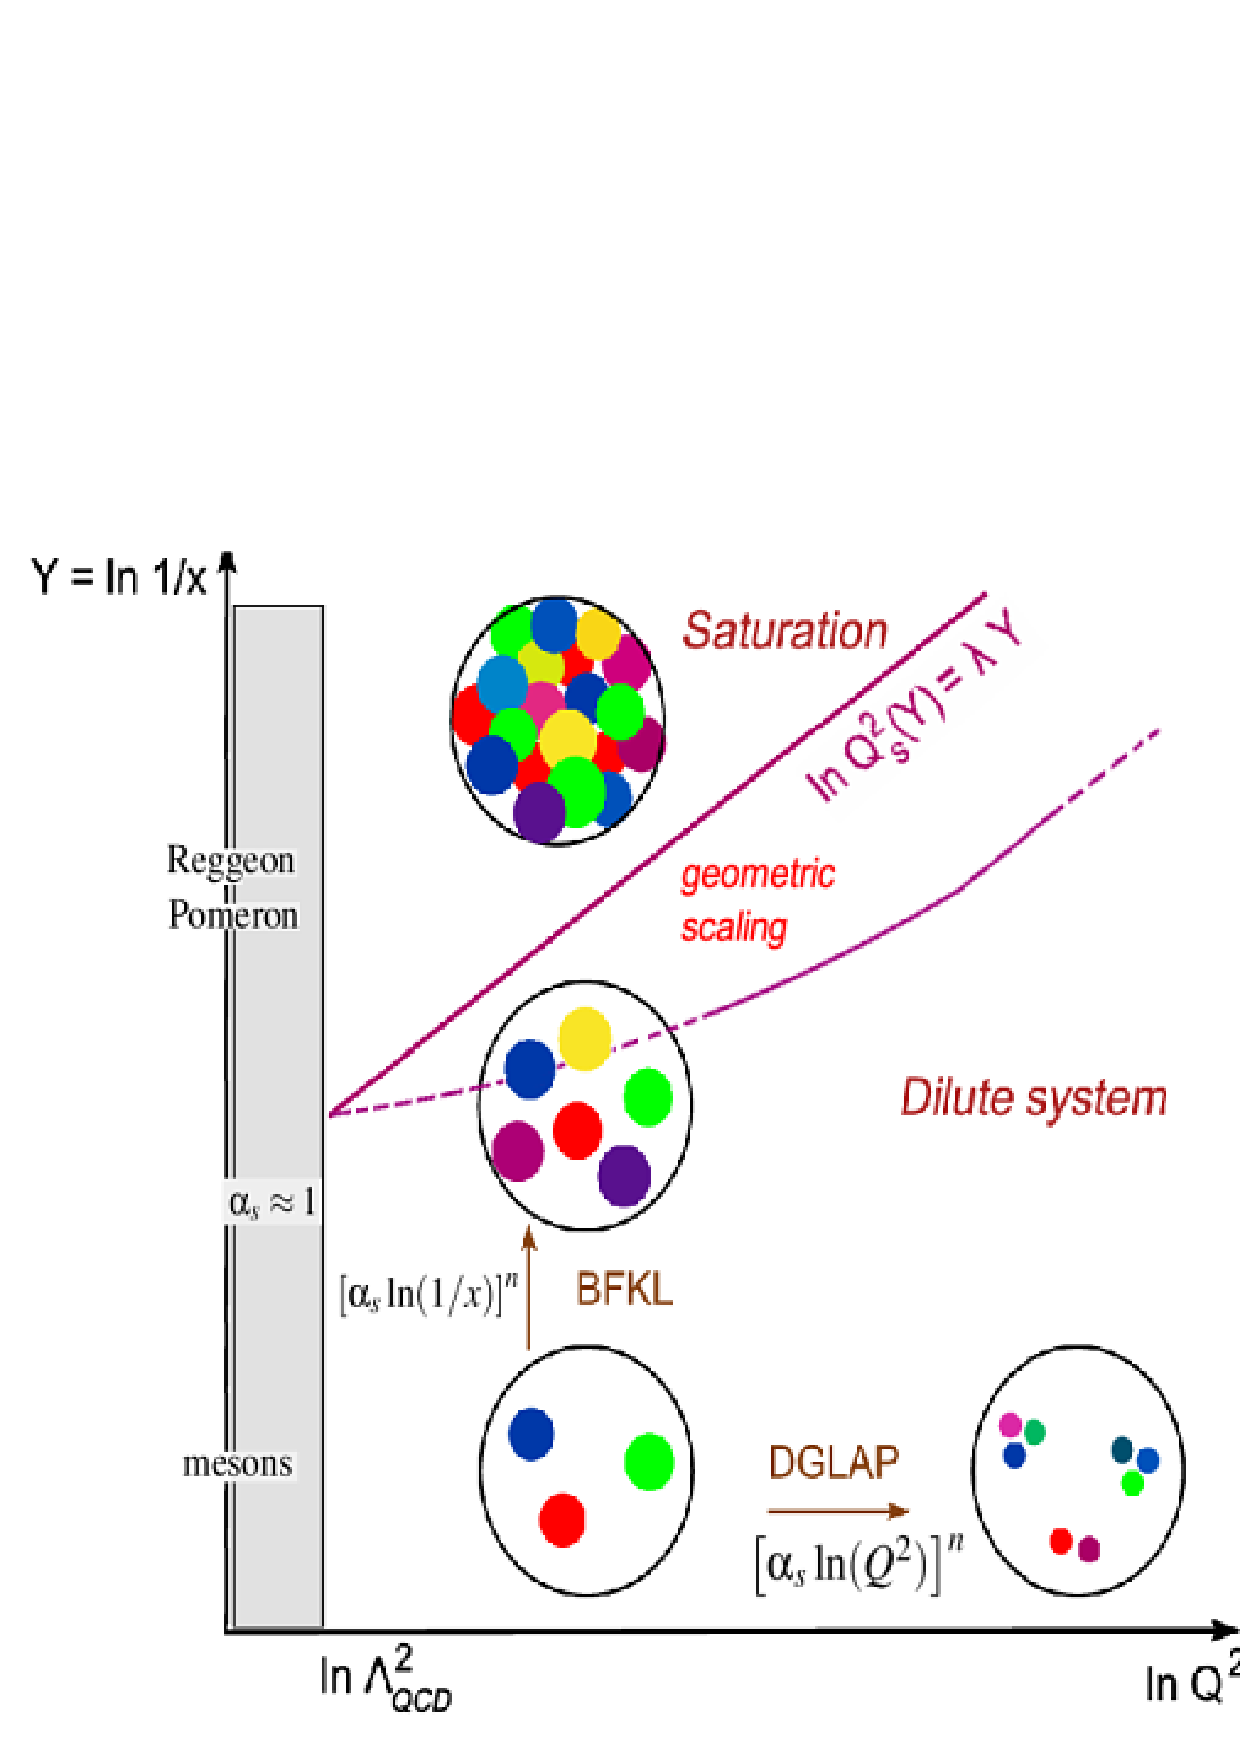
\includegraphics[width=10.cm,height=7.3cm]{introduction/y_Q2_phase_diag_cgc}
\caption{QCD phase diagram in the $1/x,Q^2$ plane (each circle represents a parton with
transverse area $\sim 1/Q^2$ and fraction $x$ of the hadron momentum).  The different evolution
regimes (DGLAP, BFKL, saturation) are indicated, as well as the saturation scale and geometric scaling
curves between the dense and dilute domains}
\label{fig:CGC_phase_diag}
%\vspace{-.4cm}
\end{figure}




\section{Quarkonia}

\end{section}

\end{chapter}






